\documentclass[11pt,graphicx,caption,rotating]{article}
\textheight=24cm
\textwidth=18cm
\topmargin=-2cm
\oddsidemargin=0cm
\usepackage[utf8x]{inputenc}
\usepackage[activeacute,spanish]{babel}
\usepackage{amssymb,amsfonts}
\usepackage[tbtags]{amsmath}
\usepackage{pict2e}
\usepackage{float}
\usepackage[all]{xy}
\usepackage{graphics,graphicx,color,colortbl}
\usepackage{times}
\usepackage{subfigure}
\usepackage{wrapfig}
\usepackage{multicol}
\usepackage{cite}
\usepackage{url}
\usepackage[tbtags]{amsmath}
\usepackage{amsmath,amssymb,amsfonts,amsbsy}
\usepackage{bm}
\usepackage{algorithm}
\usepackage{algorithmic}
\usepackage[centerlast, small]{caption}
\usepackage[colorlinks=true, citecolor=blue, linkcolor=blue, urlcolor=blue,breaklinks=true]{hyperref}

\begin{document}
\begin{titlepage}
\begin{center}
{\huge \textbf{Bitácora. Laboratorio De Circuitos de RF}}\\[6cm]
{\Large \textbf{Elaborado por:}}\\
{\Large Joan Sebastian Ligarreto Código: $261720$}\\
{\Large David Ricardo Martínez Hernández Código: $261931$}\\
{\Large Oscar Andres Urbano Vallejo Código: $261683$}\\[7cm]
{\Large \textbf{Circuitos de Radio Frecuencia}}\\[6cm]
{\Large Universidad Nacional de Colombia}\\
{\Large Facultad de Ingeniería}\\
{\Large Bogotá}\\
{\Large 2013}\\
\date{}
\end{center}
\end{titlepage}
\tableofcontents
\listoftables
\listoffigures

\newpage

\floatname{algorithm}{Algoritmo}

\section{Laboratorio 1: Amplificador Banda ancha}

\subsection{Prelaboratorio}\label{Prelaboratorio}
\noindent
\begin{figure}[H]
	\centering
		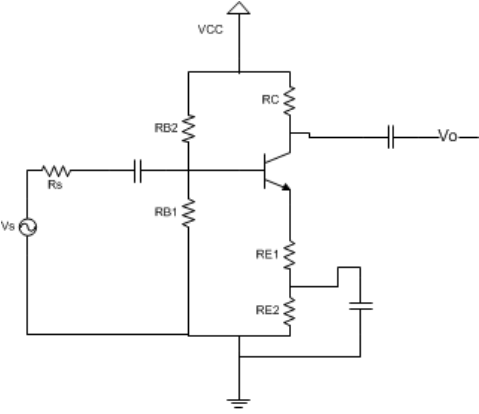
\includegraphics[scale=0.4]{circuit_lab_1a.png}
	\caption{Circuito sugerido para la práctica $1$}
	\label{fig1}
\end{figure}
\noindent
La polarización del amplificador con emisor degenerado se inicia bajo la consideración: \textbf{\textit{El voltaje en la resistencia $R_{B_{1}}$ deber ser $\frac{1}{10}$ del voltaje $V_{CC}$}}:
\begin{equation}
 V_{R_{B_1}}= 0.1*12V
\label{ecu1}
\end{equation}
\noindent
Por tanto el divisor de tensiones debe ser:
\begin{equation}
 \frac{R_{B_1}}{R_{B_1}+R_{B_2}}  = 0.1
\label{ecu2}
\end{equation}
\noindent
De donde $R_{B_2}= 9*R_{B_1}$.\\ Se establece $R_{B_2}= 68 k\Omega$ por tanto $R_{B_1}=7.5 k\Omega$ (valores normalizados).\\
Se fija el punto de polarización en $I_C= 2\ \ mA$ y $V_{CE}= 6\ \ V$, para obtener esto se despeja la resistencia de emisor en DC del lazo \textbf{$V_{CC}$–base emisor-tierra}:
\begin{equation}
 V_{TH} - 0.7= I_C\frac{R_{TH}}{\beta}+ \alpha I_{E} R_{E}
\label{ecu3}
\end{equation}
\begin{equation}
  V_{TH}= 1.1921 V,\ \ R_{TH}= 6.755 k\Omega
\label{ecu4}
\end{equation}
\begin{equation}
 \beta= 300,\ \ \alpha= \frac{301}{300}
\label{ecu5}
\end{equation}
\noindent
Al despejar se obtiene:
\begin{equation}
 R_E= 0.222 k\Omega
\label{ecu6}
\end{equation}
\noindent
Se espera tener un $V_{CE}=6 V$ por tanto haciendo el lazo de \textbf{$V_{CC}$-colector-emisor-tierra}:
\begin{equation}
 12 - R_C * I_C - V_{CE} - R_E * I_E=0
\label{ecu7}
\end{equation}
\begin{equation}
 R_E + R_C = 3 k\Omega
\label{ecu8}
\end{equation}
\noindent
de donde $R_C$ normalizado $R_C= 2.7 k\Omega$.\\
Ahora se sabe que $R_E = R_{E_1} +R_{E_2}$ y se utiliza la consideración de la ganancia aproximada para el emisor degenerado en este caso  $A_V= -\frac{R_C}{R_{E_1}}$   de donde se obtiene $R_{E_1}$ normalizado $R_{E_1}=120 \Omega$ por tanto $R_{E_2} = 100 \Omega$ .\\
Con las resistencias normalizadas el nuevo punto de operación es:
$$ I_C= 2.023  mA\ \ V_{CE}=  6.0914 V$$
\noindent
La ganancia:
\begin{equation}
 A_V  = \frac{{V_0 }}{{V_B }} =  - \frac{{\left( {\beta r_0  - {\mathop{\rm R}\nolimits} _E } \right)R'_L }}{{r_\pi  \left( {R'_L  + R_E  + r_0 } \right) + R_E \left( {R'_L \left( {\beta  + 1} \right)r_0 } \right)}}
\label{ecu9}
\end{equation}
\noindent
$A_V=-20.19$.

\subsubsection{Simulación}
\begin{figure}[H]
	\centering
		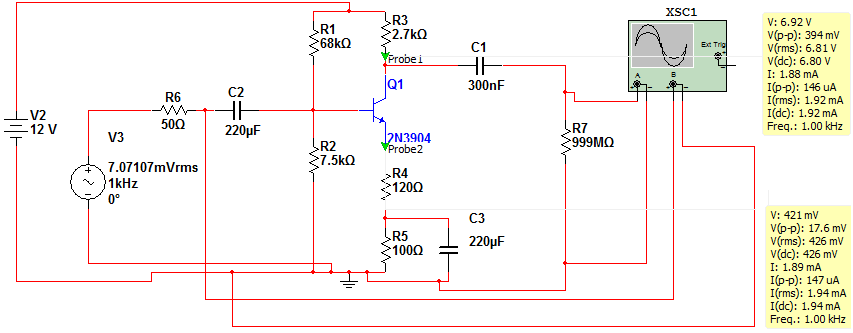
\includegraphics[scale=0.4]{circuit_lab_1.png}
	\caption{Circuito simulado para la práctica $1$.}
	\label{fig2}
\end{figure}

\begin{figure}[H]
	\centering
		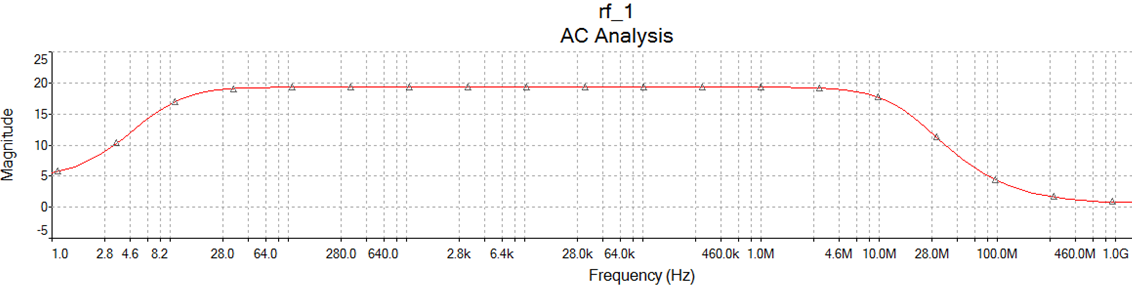
\includegraphics[scale=0.4]{simulation_lab_1.png}
	\caption{Gráfica de Ganancia en función de la frecuencia para la práctica $1$.}
	\label{fig3}
\end{figure}

\subsection{Laboratorio}
\noindent
Como el prelaboratorio (ver  ~\ref{Prelaboratorio}) no funciono se realizo un nuevo punto de polarización (ver ~\ref{Prelaboraotiro_2}).

\subsubsection{Prelaboratorio 2}\label{Prelaboraotiro_2}
\noindent
Se tomo nuevamente el circuito sugerido por el profesor Figura \ref{fig1}, utilizando el mismo criterio descrito en el prelaboratorio anterior (ver  ~\ref{Prelaboratorio}).\\
De acuerdo a las ecuaciones (\ref{ecu1}) y (\ref{ecu2}) se determinaron los valores de $R_{B_2} = 68 k\Omega$ y $R_{B_1} = 7.5 k\Omega$ (valores normalizados).\\
Se fijó el punto de polarización en $I_C= 7 mA$ y $V_{CE}= 5V$.\\
Con la ecuación (\ref{ecu3}) se determinó el valor de $R_E = 47.62 \Omega$.\\
Para obtener el punto de polarización de $V_{CE} = 5 V$ se utilizó la ecuación (\ref{ecu7}) y se encontró el valor de $R_C = 0.9524 k\Omega$ que normalizada es $R_C = 1 k\Omega$.\\
de donde $R_C$ normalizado $R_C= 2.7 k\Omega$.\\
Ahora se sabe que $R_E = R_{E_1} +R_{E_2}$ y se utiliza la consideración de la ganancia aproximada para el emisor degenerado en este caso  $A_V= -\frac{R_C}{R_{E_1}}$   de donde se obtiene $R_{E_1}=43 \Omega$ y $R_{E_2} = 6.2 \Omega$.
\begin{figure}[H]
	\centering
		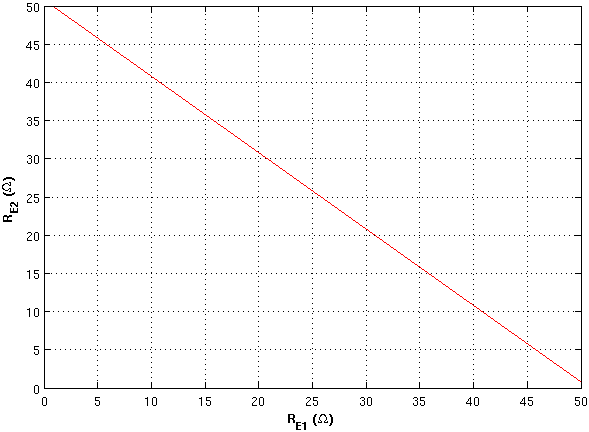
\includegraphics[scale=0.65]{resultado_re2.png}
	\caption{$R_{E_2}$ en función de $R_{E_1}$.}
	\label{fig6}
\end{figure}
\noindent
Con las resistencias normalizadas el nuevo punto de operación es:
$$ I_C= 6.8454 mA\ \ V_{CE}= 4.8167 V$$
\noindent
La ganancia:
\begin{equation}
 A_V  = \frac{{V_0 }}{{V_B }} =  - \frac{{\left( {\beta r_0  - {\mathop{\rm R}\nolimits} _E } \right)R'_L }}{{r_\pi  \left( {R'_L  + R_E  + r_0 } \right) + R_E \left( {R'_L \left( {\beta  + 1} \right)r_0 } \right)}}
\label{ecu10}
\end{equation}
\noindent
$A_V=-21.2147$.

\subsubsection{Simulación}
\noindent
\begin{figure}[H]
	\centering
		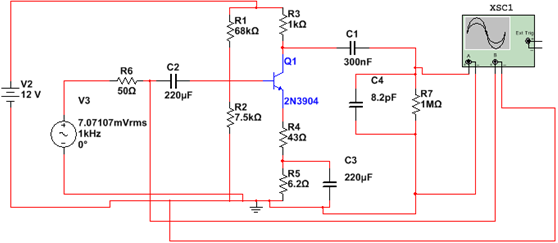
\includegraphics[scale=0.65]{circuit_lab_1b.png}
	\caption{Circuito simulado para la práctica $1$.}
	\label{fig4}
\end{figure}

\begin{figure}[H]
	\centering
		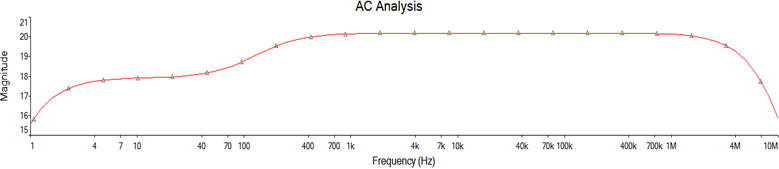
\includegraphics[scale=0.65]{simulation_lab_1b.png}
	\caption{Gráfica de Ganancia en función de la frecuencia para la práctica $1$.}
	\label{fig5}
\end{figure}

\subsubsection{Resultados Obtenidos}
\noindent
Se realizó el montaje de la Figura \ref{fig4} y se obtuvieron los siguientes resultados.\\
Para la polarización se obtuvo:

\begin{table}[H]
	\centering
\begin{tabular}{|c|c|}\hline
\textbf{Elemento} & \textbf{Medición} \\ \hline
$V_{CC}$ & $5.58V$ \\ \hline
$V_{R_C}$ & $6.5 V$ \\ \hline
$V_{CE}$ & $5.58V$ \\ \hline
$R_C$ & $0.983 k\Omega$ \\ \hline
$R_{E_1}$ & $0.983 k\Omega$ \\ \hline
$R_{E_2}$ & $0.983 k\Omega$ \\ \hline
$R_1$ & $0 k\Omega$ \\ \hline
$R_2$ & $0 k\Omega$ \\ \hline
$I_C$ & $6.6124 mA$ \\ \hline
    \end{tabular}
	\caption{Medidas obtenidas para la práctica $1$.}
	\label{tab1}
\end{table}
\noindent
Medidas obtenidas de ganancia a una frecuencia determinada:
\begin{table}[H]
	\centering
\begin{tabular}{|c|c|}\hline
 \textbf{Frecuencia (Hz)} & \textbf{Ganancia} \\ \hline
$100$ & $9.19$ \\ \hline
$230$ & $14.67$ \\ \hline
$250$ & $15$ \\ \hline
$300$ & $15.64$ \\ \hline
$1k$ & $17.9$ \\ \hline
$10k$ & $18.095$ \\ \hline
$100k$ & $18.3$ \\ \hline
$200k$ & $19.61$ \\ \hline
$800k$ & $19.25$ \\ \hline
$1M$ & $19.03$ \\ \hline
$2M$ & $19.07$ \\ \hline
$3M$ & $18.24$ \\ \hline
$4M$ & $17.5$ \\ \hline
$5M$ & $16$ \\ \hline
$6M$ & $14.6$ \\ \hline
$6.8M$ & $14.26$ \\ \hline
$7M$ & $13.3$ \\ \hline
    \end{tabular}
	\caption{Tabla de  Ganancia en función de la frecuencia para la práctica $1$.}
	\label{tab2}
\end{table}

\begin{figure}[H]
	\centering
		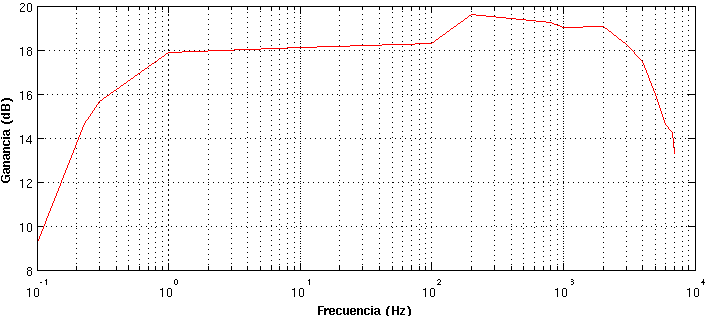
\includegraphics[scale=0.65]{resultado_ganancia.png}
	\caption{Resultado de la ganancia del circuito de la Figura \ref{fig4}.}
	\label{fig7}
\end{figure}
\noindent
Los valores son muy similares a los obtenidos en el script de matlab \textit{amplificador\_ banda.m}.\\
¿Explique los efectos de las sondas sobre la respuesta en frecuencia?\\
Las sondas limitan la frecuencia de corte superior $F_{H3}$ de un amplificador de banda ancha, debido al efecto capacitivo asociado al estar atenuadas, de $17 pF$ aproximadamente, además se tiene un efecto resistivo que varía con la frecuencia que se maneje.
¿Explique como el factor de calidad de los elementos del circuito afecta la respuesta en frecuencia de todo
el sistema?\\
El factor de calidad de cada uno de los componentes empleados para un montaje de radiofrecuencia  determina que tan bueno será su funcionamiento en la frecuencia de trabajo y que tanto pueden llegar a disipar o almacenar energía como se espera, de manera que no se agreguen efectos no deseados, puesto que esto compromete la respuesta en frecuencia, ya que se afectan las consideraciones iniciales.

\subsection{Conclusiones}
\begin{itemize}
 \item Incluyendo una resistencia de degeneración de un valor bajo para un amplificador BJT de emisor común, es posible obtener un eficiente manejo del ancho de banda y un buen control de la ganancia.
 \item El diseño de circuitos en radiofrecuencia requiere tener en consideración los efectos inductivos y capacitivos de cada componente, con el objetivo de trabajar sobre modelos confiables que incluyan todas las variables que se ven involucradas en los análisis de estos circuitos.
 \item Los circuitos en comunicaciones se manejan en alta frecuencia, así que es importante determinar el ancho de banda de un amplificador en RF, considerando siempre que la ganancia obtenida va a estar en relación inversa con el ancho de banda.
\end{itemize}

\section{Laboratorio 2: Amplificador selectivo en frecuencia}

\subsection{Prelaboratorio}
\noindent
\begin{figure}[H]
	\centering
		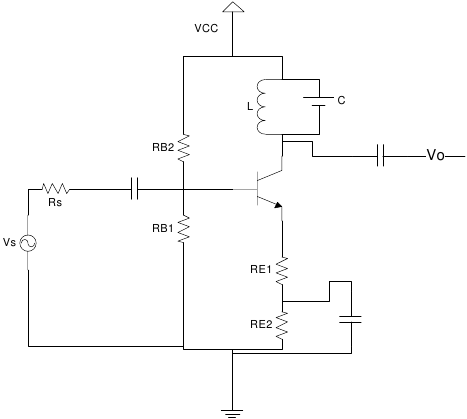
\includegraphics[scale=0.5]{circuit_lab_2.png}
	\caption{Circuito sugerido para la práctica $2$}
	\label{fig8}
\end{figure}
\noindent
La polarización del amplificador con emisor degenerado se inicia bajo la consideración: \textbf{\textit{El voltaje en la resistencia $R_{B_{1}}$ deber ser $\frac{1}{10}$ del voltaje $V_{CC}$}}. De acuerdo a las ecuaciones (\ref{ecu1}) y (\ref{ecu2}) se determinaron los valores de $R_{B_2} = 68 k\Omega$ y $R_{B_1} = 7.5 k\Omega$ (valores normalizados).\\
La frecuencia de resonancia seleccionada para el grupo es de $4,4 Mhz$ con esto se calculan los valores de $C$ y $L$ por medio de la ecuación de para la resonancia de un circuito en paralelo:
\begin{equation}
 f_0=\frac{1}{2 \pi \sqrt{L C}}
\label{ecu11}
\end{equation}
\noindent
Utilizando la ecuación anterior se determino un valor de $L$ talque tuviera un capacitor comercial, los valores seleccionados fueron $L=22 \mu H$ y $C=59 pF$.\\
Como la ganancia aproxima para este tipo de configuración es aproximadamente:
\begin{equation}
 A_V \approx \frac{-R'_L}{R_E}
\label{ecu12}
\end{equation}
\noindent
donde:\\
$R'_L=R_C \parallel R_L$.\\
Para este caso en particular $R'_L = R_C=L\parallel C$ dada esta relación y poder obtener el valor de esta resistencia se desprecio los efectos resistivos del capacitor, solo se tiene en cuenta los correspondientes a la bobina procediendo de la siguiente manera:
\begin{eqnarray}
 R'_L & = & R_{L_{Parallel}} \label{ecu13}\\
 R_{L_{Parallel}} & = & R_{L_{Serie}}\left( {1 + Q^2 } \right) \label{ecu14}\\
 R_{L_{Serie}} & = & \frac{\omega _0 L}{Q}\label{ecu15}
\end{eqnarray}
\noindent
al reemplazar la ecuación (\ref{ecu14}) en la ecuación (\ref{ecu15}), se obtiene
\begin{equation}
 R_{L_{Parallel}}=\frac{\omega _0 L}{Q}\left( {1 + Q^2 } \right)
\label{ecu16}
\end{equation}
\noindent
De acuerdo a la ecuación anterior y con el valor de $Q=50$ $R_{L_{Parallel}}=4.8613 k\Omega$. Por consiguiente y de acuerdo a la ecuación (\ref{ecu12}) el valor de $R_E=270 R_C \Rightarrow R_{E_1}=18.0047 \Omega$ que normalizado es $R_{E_1}=18\Omega$.\\
Para la polarización se utilizo $I_C=12 mA$, $R_1=68 k\Omega$, $R_2=7.5 k\Omega$, $R_{E_2}=3.6 \Omega$.

\subsubsection{Simulación}

\begin{figure}[H]
	\centering
		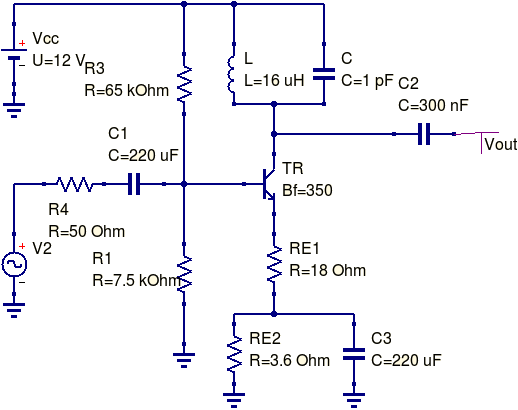
\includegraphics[scale=0.6]{circuit_lab_2a.png}
	\caption{Circuito simulado para la práctica $2$.}
	\label{fig9}
\end{figure}

\begin{figure}[H]
	\centering
		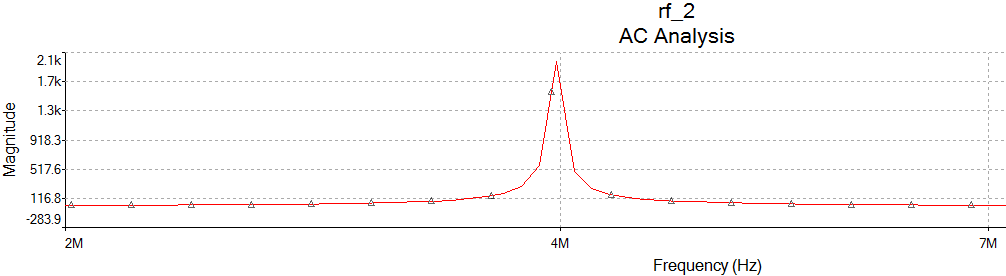
\includegraphics[scale=0.45]{simulation_lab_2.png}
	\caption{Gráfica de Ganancia en función de la frecuencia para la práctica $2$.}
	\label{fig10}
\end{figure}

\subsection{Laboratorio}
\noindent
\subsubsection{Resultados Obtenidos - Parte 1}
\noindent
De acuerdo al montaje de la Fig \ref{fig10} se obtuvieron prácticamente los siguientes valores:
\begin{table}[H]
	\centering
\begin{tabular}{|c|c|}\hline
 \textbf{Elemento} & \textbf{Valor} \\ \hline
 $V_{CC}$ & $11.98V$ \\ \hline
 $F_R$ & $4.47MHz$ \\ \hline
 $A_V$ & $436.046$ \\ \hline
 $V_O$ & $15.6V$ \\ \hline
 $R_1$ & $68.8K\Omega$ \\ \hline
 $R_2$ & $7.49K\Omega$ \\ \hline
 $R_{E_1}$ & $18.4\Omega$ \\ \hline
 $R_{E_2}$ & $2.4\Omega$ \\ \hline
 $I_{C_Q}$ & $11.59mA$ \\ \hline
 $V_{CE_Q}$ & $11.96V$ \\ \hline
    \end{tabular}
	\caption{Valores obtenidos en la práctica.}
	\label{tab3}
\end{table}
\noindent
Cuando se polarizaba el transistor con una señal AC de $V_{gen}= 100 mV$ tenia una caída a $34.4 mV$.\\
Los valores son muy similares a los obtenidos en la simulación y el script de matlab \textit{resonance.m}.\\
¿Qué propiedades observan del circuito?\\
Se observa una ganancia grande, con un ancho de banda estrecho,  debido a que la idea era poner en oscilación el tanque a la frecuencia solicitada, logrando una selección de la frecuencia en la cual operaba el montaje.\\
¿Qué puede decir acerca de las propiedades observadas?\\
Acerca de las propiedades observadas puede decirse que el amplificador selectivo en frecuencia genera  cierta sensibilidad, debido a que es fácil salirse del ancho de banda especificado, además, se aprecia una alta ganancia en este punto dada por el efecto del tanque.
¿Qué tan bueno fue su cálculo del ancho de banda, explique la razón de su acierto o fallo?\\
El ancho de banda calculado fue de aproximadamente $400KHz$, semejante al valor esperado, que se calculó en $552.9KHz$ para el tanque considerado.\\
¿Qué sucede al conectar la resistencia de carga, explique a través de la teoría?\\
Al conectar la resistencia de carga se aumenta el factor de calidad del tanque pero se disminuye el ancho de banda.\\

\subsubsection{Resultados Obtenidos - Parte 2}
\noindent
Para la segunda parte del laboratorio se utilizo el mismo circuito de la Figura \ref{fig10} pero esta vez se pidió que tuviera una resonancia superior a $12MHz$, cuando se desarrollo se hizo resonar a $14.2MHz$, solo se cambio la inductancia de $22\mu H$ a $0.8\mu H$.\\
La Figura \ref{fig11} muestra la respuesta del circuito utilizando el analizador de espectros.
\begin{figure}[H]
	\centering
		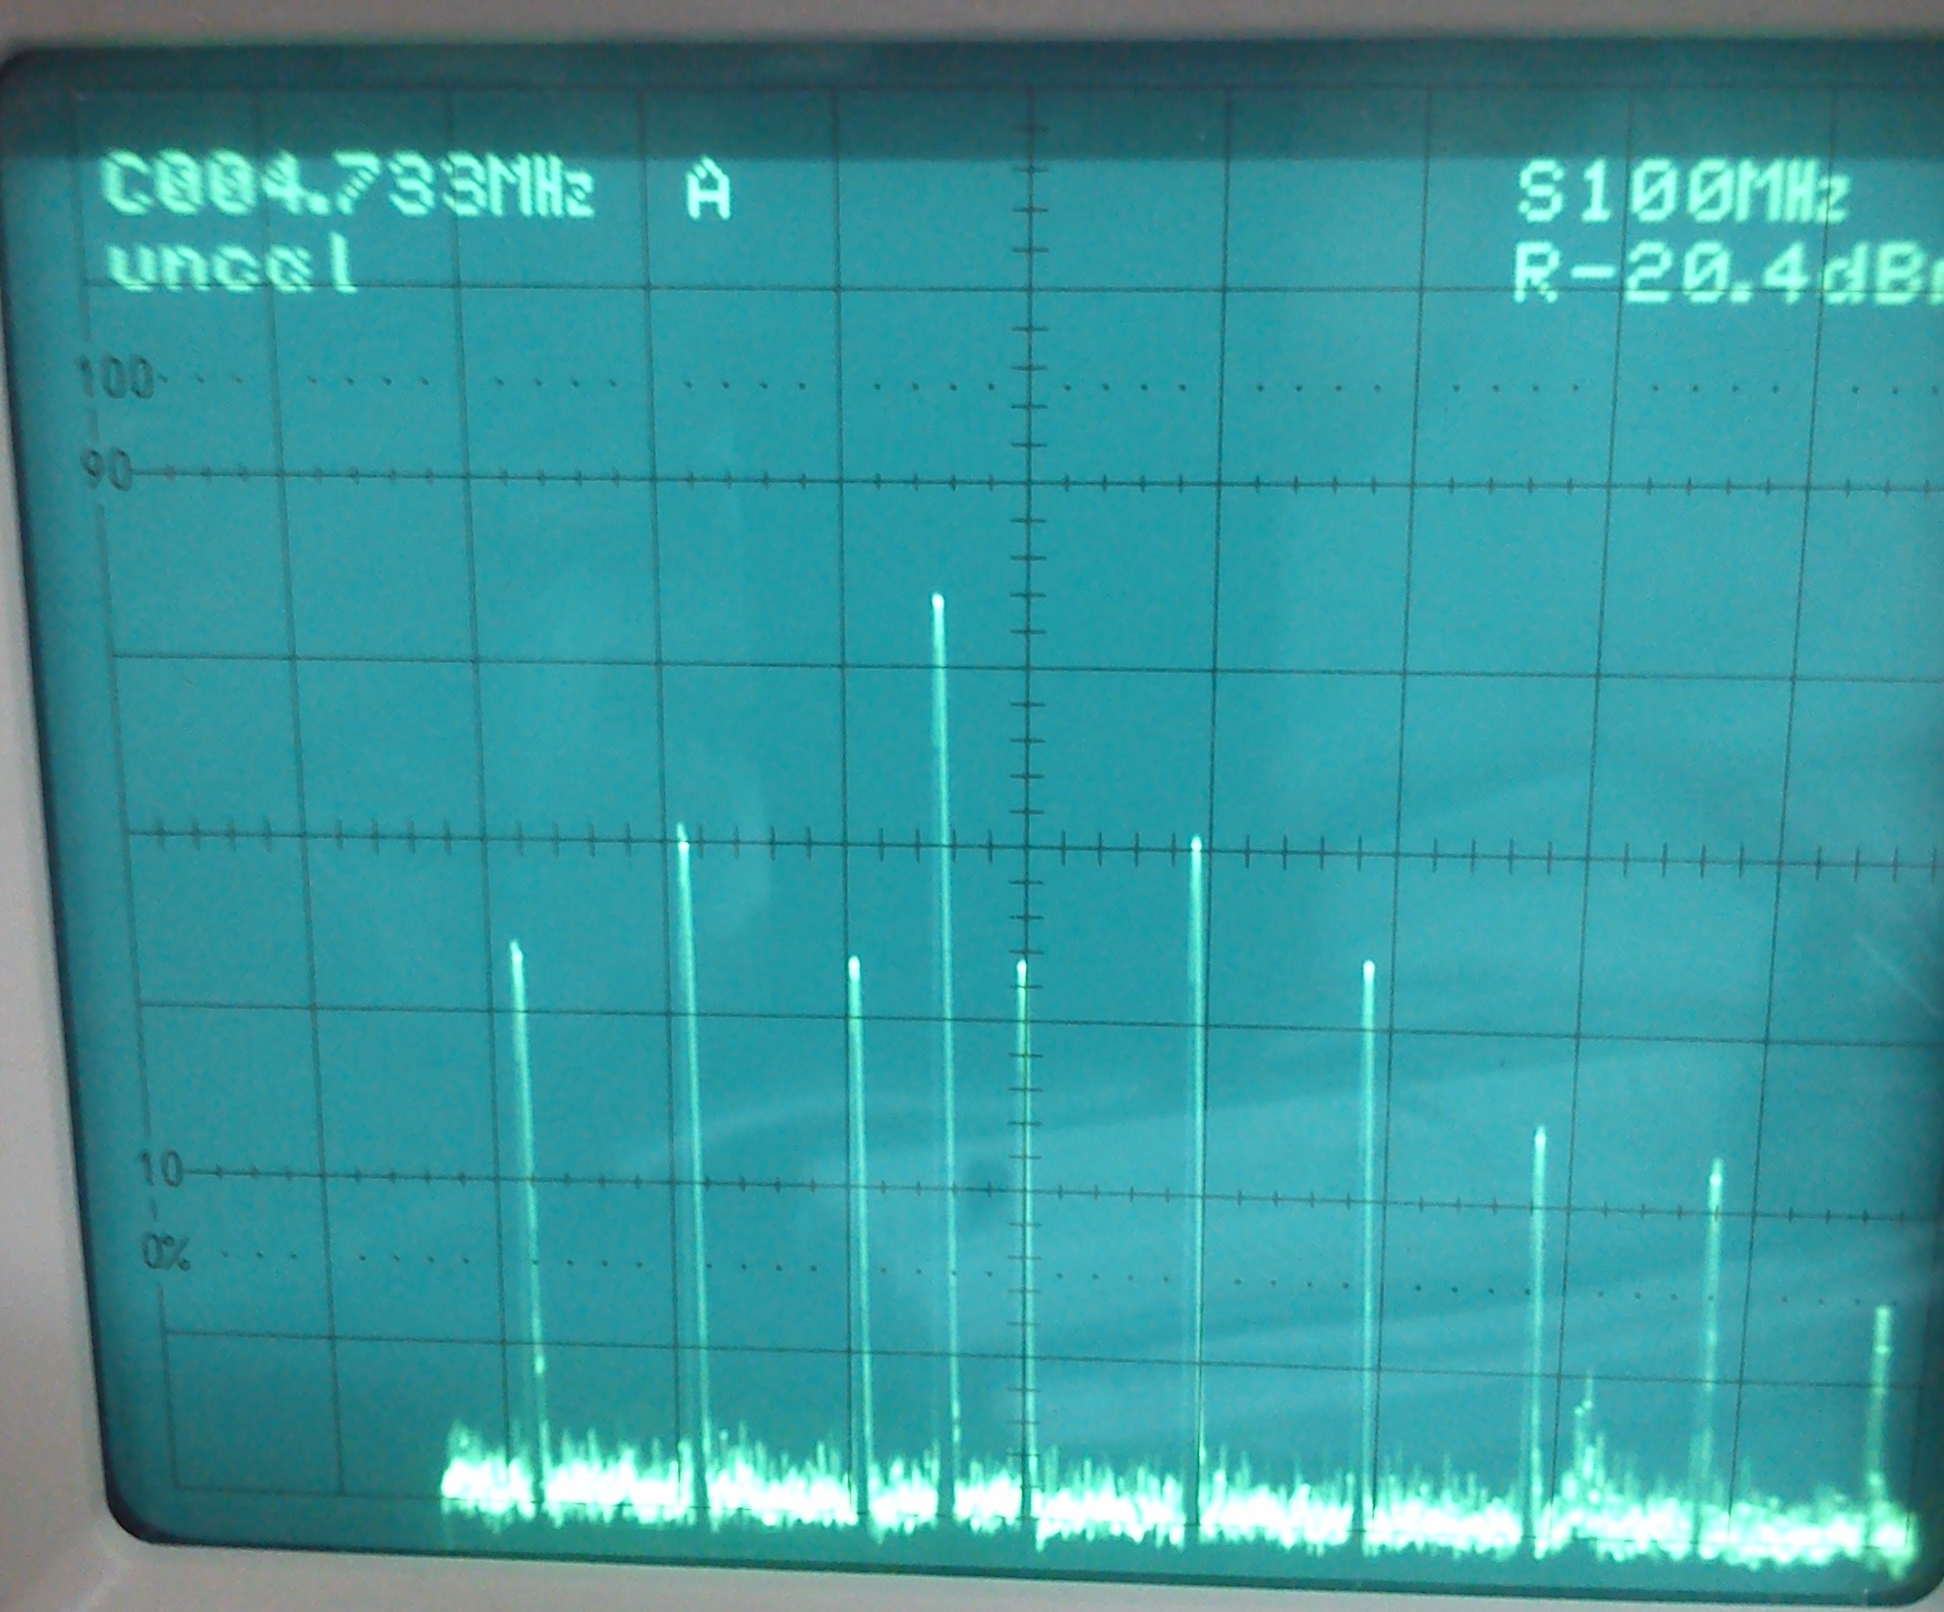
\includegraphics[scale=0.2]{thd.png}
	\caption{Salida del analizador de espectros para la práctica $2$.}
	\label{fig11}
\end{figure}
\noindent
¿Cómo deberá ser la salida del amplificador al alimentarlo con la onda cuadrada?\\
Al alimentarlo con una onda cuadrada la salida del amplificador va a resultar de tipo senoidal para la frecuencia de resonancia.
¿Es posible realizarlo con el quinto armónico?\\
Pues para ese montaje que se realizo como se puede observar en la Figura \ref{fig11}, el quinto armónico esta muy atenuado y la salida que se obtuvo no era muy buena por que el tercer armónico es mucho mayor, para poderlo hacer es necesario diseñar un filtro pasabanda para el quinto armónico.

\subsection{Conclusiones}
\begin{itemize}
 \item Se observa que el amplificador selectivo en frecuencia permite centrar una frecuencia en resonancia con alto factor de calidad y bajo ancho de banda, lo cual resulta útil en muchas aplicaciones de comunicaciones.
 \item Se encontró que los valores finales son muy similares a los obtenidos en la simulación y el script de matlab realizado, llamado \textit{resonance.m}.
 \item Es posible realizar una atenuación de todos los armónicos salvo el primero y el tercero, en base a una configuración del tanque que aumenta la frecuencia de resonancia.
 \item Es posible generar una onda senoidal a partir de una onda cuadrada realizar el circuito multiplicador.
\end{itemize}

\section{Laboratorio 3: Acoplador de impedancias}
\subsection{Prelaboratorio}
\noindent
Se siguió la recomendación del profesor descrita en la guía de laboratorio, los resultados obtenidos de los valores de condensadores y de la bobina fueron determinados por el scrip de matlab \textit{Practica\_3.m} se obtuvo lo siguiente:
\begin{table}[H]
	\centering
\begin{tabular}{|c|c|c|}\hline
 \textbf{Elemento} & \textbf{Valor} & \textbf{Valor Normalizado} \\ \hline
 $C_1$ & $20.64nF$ & $22nF$ \\ \hline
 $C_2$ & $71.18nF$ & $68nF$ \\ \hline
 $L_{acoplador}$ & $82.28nH$ & $80nH$ \\ \hline
 $L_{transistor}$ & $22 \mu H$ & $22 \mu H$ \\ \hline
    \end{tabular}
	\caption{Valores obtenidos para la Práctica $3$.}
	\label{tab4}
\end{table}

\subsubsection{Simulación}
\begin{figure}[H]
	\centering
		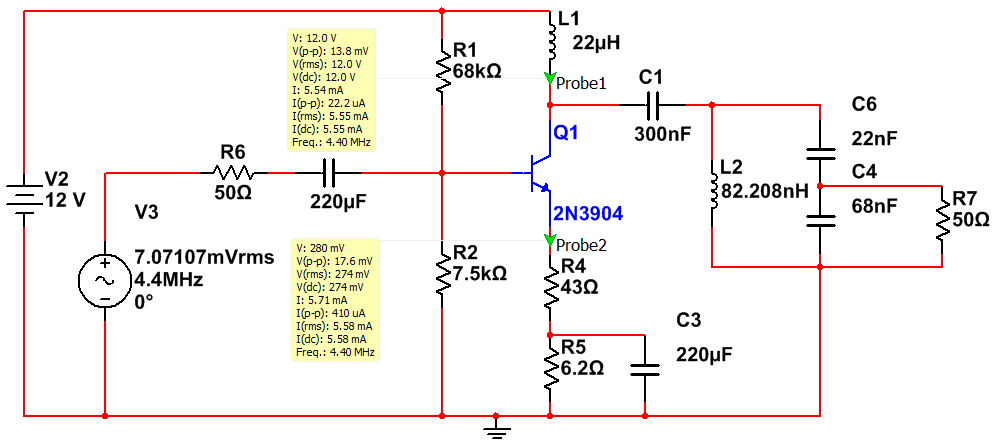
\includegraphics[scale=0.5]{circuito_lab_3.png}
	\caption{Circuito simulado para la práctica $3$.}
	\label{fig12}
\end{figure}
\begin{figure}[H]
	\centering
		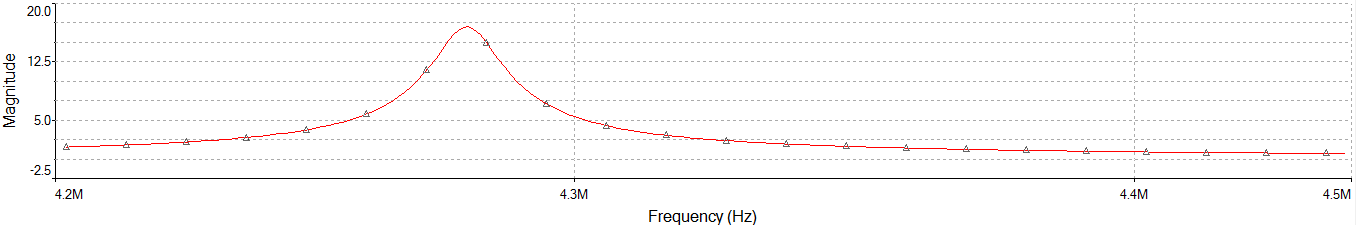
\includegraphics[scale=0.5]{simulation_lab_3.png}
	\caption{Gráfica de Ganancia en función de la frecuencia para la práctica $3$.}
	\label{fig13}
\end{figure}
\noindent
Como se puede observar en la Figura \ref{fig13} el punto de resonancia se corre aproximadamente a $4.3MHz$ cuando se normalizan los valores, esto se podrá comprobar al implementar el circuito en el laboratorio.

\subsection{Laboratorio}
\noindent
Este laboratorio no fue posible implementarlo debido a los valores poco prácticos de inductancia para la red de acople ($80 nH$), dicha inductancia no se pudo conseguir en el mercado, sin embargo se optó por fabricar una que se le acercara a su valor;  por formula de Harold Wheeler:
\begin{equation}
 L_{\left( {\mu H} \right)}  = \frac{{0.39r^2 n^2 }}{{9r + 10li}}
\label{ecu17}
\end{equation}
\noindent
La inductancia determinada por medio de dicha fórmula contó con las siguientes dimensiones: diámetro de $d=0.8 cm$ y una longitud de $l=2.2 cm$ con $n=4$ espiras, fue diseñada con núcleo de aire y cable de protoboard AWG.\\
El diseño de las bobinas no fue del todo satisfactorio, sin embargo después de algunos ajustes se consiguió que la red de acople resonara a una frecuencia de $4.5 MHz$,  mas sin embargo el amplificador funciono solo a partir de $13.5 MHz$ por dicha razón y por falta de tiempo \textbf{NO} fue imposible acoplar los dos circuitos.

\section{Laboratorio 4: Oscilador}
\subsection{Prelaboratorio}
\noindent
Para el diseño del oscilador se decidió hacer uso de valores mas comerciales para la inductancia. La mínima bobina que se pudo hallar en el mercado de un valor confiable fue de $12 \mu H$, valor con el cual se rediseño la red de acople que en este caso será utilizada como  red de realimentación.
\begin{figure}[H]
	\centering
		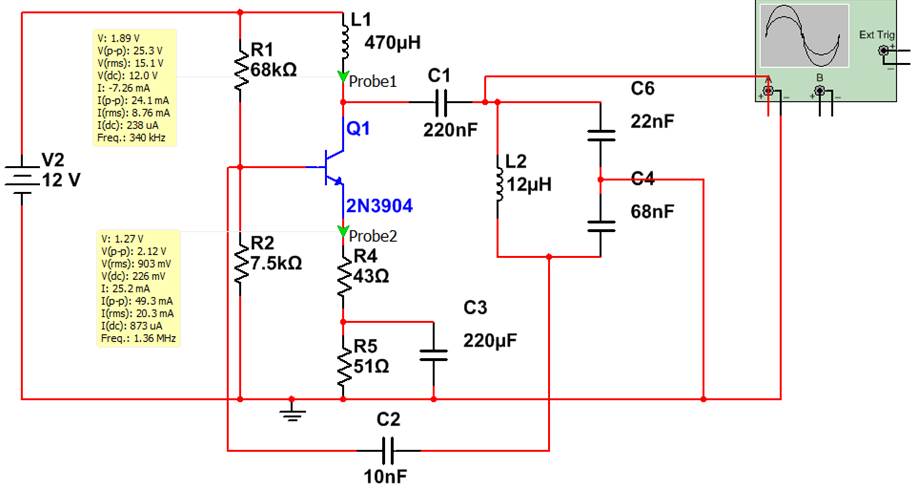
\includegraphics[scale=0.5]{circuit_lab_4.png}
	\caption{Oscilador de Colpits, circuito simulado para la práctica $4$.}
	\label{fig14}
\end{figure}
\noindent
El diseño de la red de acople fue el mismo que el que se siguió en la guía 3 de laboratorio, sin embargo en este caso se fijo la inductancia en $12\mu H$ valor para el cual la frecuencia de resonancia:
\begin{eqnarray}
 f_r & = & \frac{1}{{2\pi \sqrt {\left( {22\mu F \parallel 68nF} \right)12\mu H} }} \label{ecu18}\\
& = & 356,35 KHz
\end{eqnarray}
\noindent
Haciendo uso del circuito acoplador para realimentar por la base el amplificador de emisor degenerado, se creo el oscilador de Colpits; su simulación arrojo los siguientes datos:
\begin{figure}[H]
	\centering
		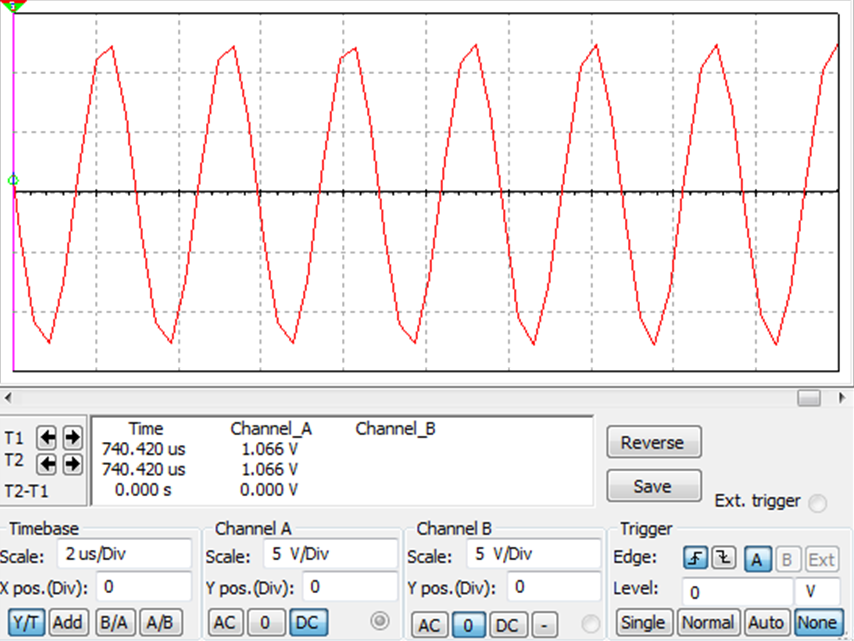
\includegraphics[scale=0.35]{simulation_lab_4.png}
	\caption{Simulacion oscilador de Colpits para la práctica $4$.}
	\label{fig15}
\end{figure}
\noindent
La onda resultante es aproximadamente senoidal cuenta con un $V_p = 12 V$ y una frecuencia $f_r= 333.33 KHz$.

\subsection{Resultados Obtenidos}
\noindent
El oscilador de colpits se implementó exitosamente, se consiguió generar una señal senoidal de $350 KHz$ de frecuencia y $10.2 V_{pp}$.

\subsection{Problemas encontrados en la implementación}
\noindent
Inicialmente se diseño el amplificador para que tuviera una alta ganancia (cercana a $20$), sin embargo a la hora de implementar el circuito se observó que el oscilador era altamente inestable pues la oscilación aumentaba hasta saturar el transistor. Teniendo en cuenta el criterio de \textbf{BarkHaussen} se bajo la ganancia hasta un valor aproximado a $10$ (variando la resistencia de emisor degenerado de $6.2 \Omega$ a $51 \Omega$), en dicho valor el producto $AB$ es mas cercano a $1$; lo cual vuelve el oscilador altamente estable.

\section{Laboratorio 5: Modulación AM}
\noindent
En esta práctica se hizo uso de el oscilador diseñado en la guía 4 y se lo utilizo para modular una señal de audio; frecuencia máxima del mensaje $20 KHz$; Al oscilador de colpits diseñado en la práctica pasada se le superpone una señal (mensaje) por la base y se obtiene la onda modulada por el colector.
\begin{figure}[H]
	\centering
		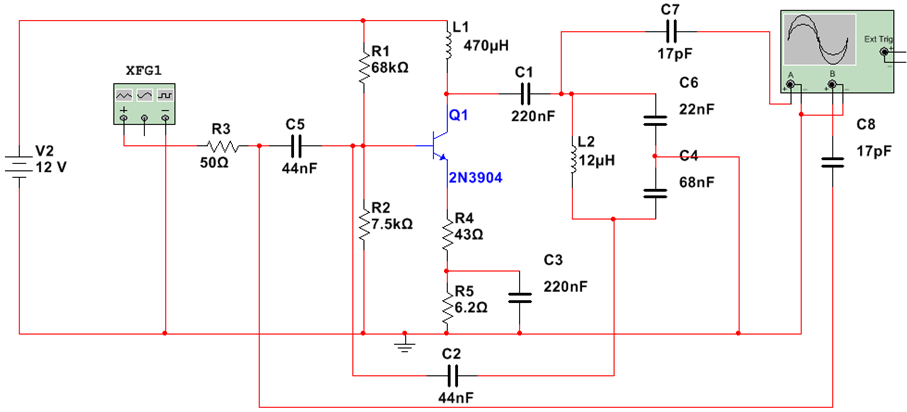
\includegraphics[scale=0.5]{circuit_lab_5.png}
	\caption{Modulador AM simulado para la práctica $4$.}
	\label{fig16}
\end{figure}
\begin{figure}[H]
	\centering
		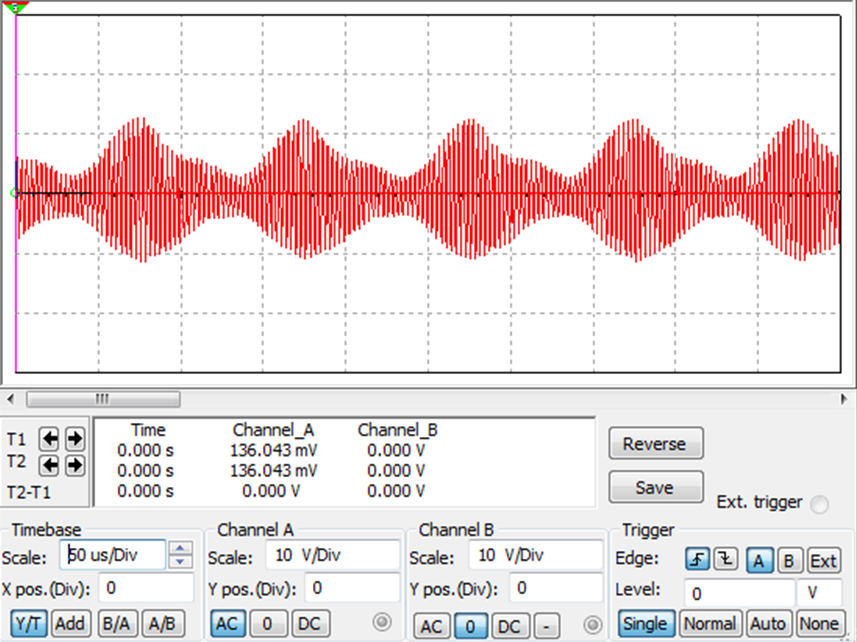
\includegraphics[scale=0.35]{simulation_lab_5.png}
	\caption{Simulación Modulador AM, mensaje $10KHz$ portadora $350 KHz$.}
	\label{fig17}
\end{figure}
\noindent
Del circuito implementado en el laboratorio se puede decir que para que la modulación sea optima la señal que entra por la base no debe ser mayor a $1 V_p$  pues de ser así se satura el transistor y el circuito deja de modular. La onda portadora tiene una frecuencia de $350 KHz$ lo cual asegura una buena transmisión para un mensaje comprendido entre  entre $16 Hz$ y $20 KHz$ (señal de audio).

\section{Proyecto Final: Transmisión de audio por medio de la red eléctrica}
\subsection{Parte 1: Acoplador}
\begin{figure}[H]
	\centering
		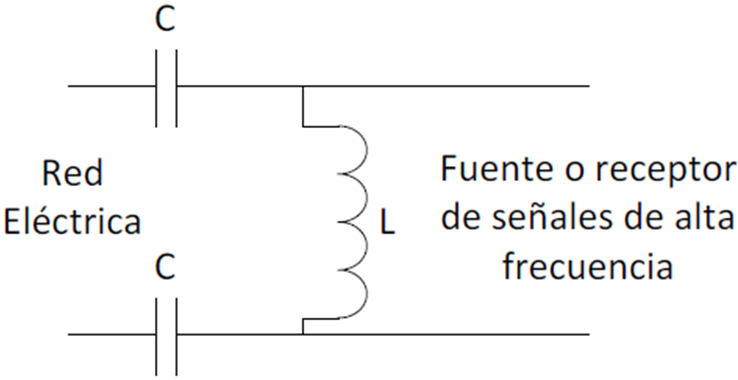
\includegraphics[scale=0.35]{acoplador.png}
	\caption{Acoplador para la red eléctrica.}
	\label{fig18}
\end{figure}
\noindent
Para el diseño del acoplador a la red eléctrica se calculó la función de transferencia :
\begin{eqnarray}
 \frac{v_O}{v_i} & = & \frac{s^{2}CL}{s^2CL +2} \label{ecu19}\\
 & = & \frac{s^{2}\frac{CL}{2}}{s^2 \frac{CL}{2} +1} \label{ecu20}
\end{eqnarray}
\noindent
Se observa que la frecuencia de resonancia es:
\begin{equation}
 f_{r} = \frac{1}{2 \pi \sqrt{L\frac{C}{2}}}
\end{equation}
\noindent
Para $L= 33 \mu H$ y $C= 5.6 nF$ se obtiene una $f_r = 523.5 KHz$.\\
Como se observa de la figura \ref{fig19} la red de acople actúa como un filtro pasa altos; a la frecuencia de resonancia  la atenuación es mínima, por tal motivo se busco que la frecuencia de la portadora del modulador y la frecuencia de resonancia de la red de acople fueran similares.
\begin{figure}[H]
	\centering
		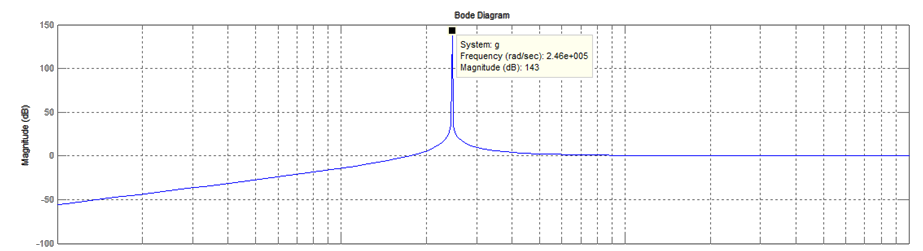
\includegraphics[scale=0.5]{bode.png}
	\caption{Función de transferencia acoplador.}
	\label{fig19}
\end{figure}

\subsection{Parte 2: Envío de audio}
\noindent
Finalmente después de implementar los circuitos de modulador y el acoplador se observó que el modulador en la práctica modula en una frecuencia base de $370 KHz$;  para esta frecuencia la red de acople tiene una atenuación bastante buena $0.8$. Así pues se espera que al propagar la onda modulada a esta frecuencia se aproveche al máximo la función de transferencia del acoplador consiguiendo a la salida de la red eléctrica una buena señal para ser demodulada y amplificada.

\bibliographystyle{ieeetran}
\begin{thebibliography}{99}
\bibitem{sedra} Jaeger, Richard C. \& Blalock, Travis N.
{\em "`Microelectronic Circuit Desing"'}.
McGraw-Hill, Fourth Edition, 1999.

\bibitem{sedra} Sedra, Adel S. \& Smith, Kenneth C.
{\em "`Circuitos Microelectrónicos"'}.
Oxford University Press, Cuarta Edición, 1999.
\end{thebibliography}
\end{document}